\chapter{Modeling with BPMN}

Business Process Model and Notation (BPMN) is a graphical representation for specifying business processes in a workflow. BPMN is designed to be easily understandable by all business stakeholders, from the business analysts who create and refine the processes to the technical developers responsible for implementing them, and finally, to the business people who manage and monitor those processes. BPMN serves as a standardized bridge between the business process design and its implementation, ensuring that everyone involved has a clear and consistent understanding of the process flow.

\section{Key Elements of BPMN}

BPMN consists of several key elements that help in modeling business processes. These elements include activities, events, gateways, and sequence flows.
\begin{figure}[h!]
    \centering
    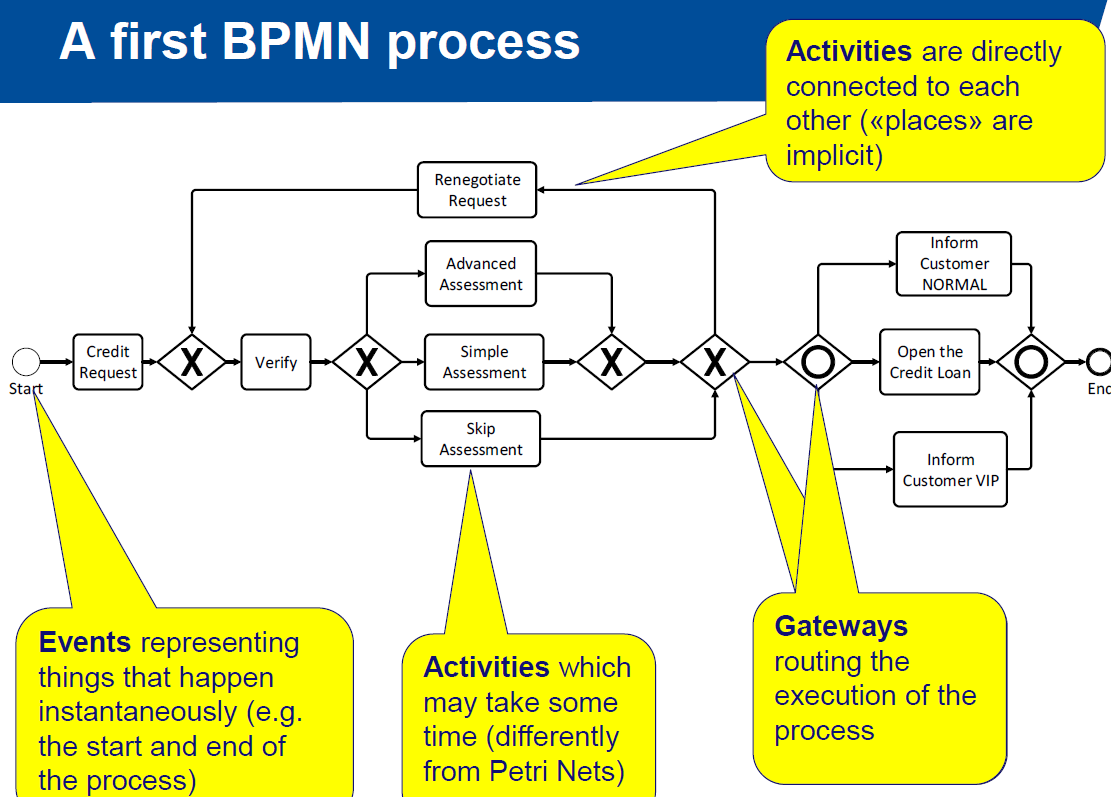
\includegraphics[width=0.75\linewidth]{capitolo 9/1.png}
\end{figure}

\subsection{Activities}

Activities are the fundamental units of work within a BPMN process. Unlike Petri Nets, where activities are connected through places, BPMN activities are directly connected to each other. This direct connection simplifies the diagram and makes it more intuitive to understand. Activities in BPMN can take some time to complete, which is a notable difference from Petri Nets, where activities are often considered instantaneous.
\begin{figure}[h!]
    \centering
    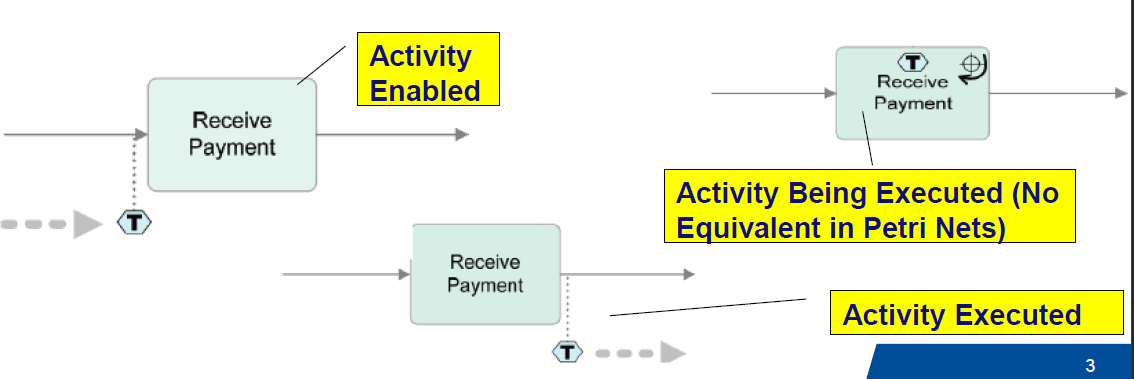
\includegraphics[width=0.75\linewidth]{capitolo 9/2.png}
\end{figure}
\subsection{Events}

Events in BPMN represent occurrences that happen instantaneously during the process. These can include the start and end of the process, as well as intermediate events that occur between activities. Events are crucial for triggering the flow of the process and can significantly influence the sequence of activities.

\subsection{Gateways}

Gateways in BPMN control the flow of the process by routing the execution based on certain conditions. They act as decision points where the process can split into multiple paths or merge from multiple paths. There are three basic types of gateways: exclusive, inclusive, and parallel.

\section{Token Semantics}

In BPMN, the concept of a token is used to track the state of a process instance. When a process instance is created, a token is generated by the start event. This token traverses the sequence flow, enabling and executing activities as it moves along. Once an activity is executed, a token is produced, which continues to flow until it is eventually destroyed by an end event.

The presence of a token before an activity indicates that the activity is enabled and ready for execution. This mechanism ensures that activities are executed in the correct sequence and that the process flow is maintained. Unlike Petri Nets, BPMN does not have an equivalent concept for tokens, making it a unique feature of BPMN.

\section{Gateways in BPMN}

Gateways in BPMN serve as control points that manage the flow of tokens through the process. They can split the flow into multiple paths or merge multiple paths into one. The behavior of gateways is determined by their type: exclusive, inclusive, or parallel.
\begin{figure}[h!]
    \centering
    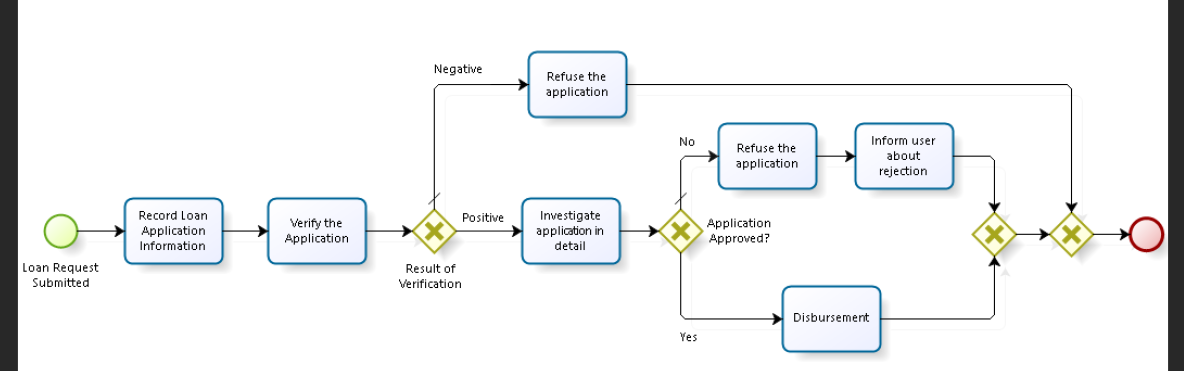
\includegraphics[width=1\linewidth]{capitolo 9/6.png}
\end{figure}

\subsection{Exclusive Gateways (XOR)}

Exclusive gateways, also known as XOR gateways, allow the process to choose between alternative paths based on certain conditions. When a token reaches an XOR split, the conditions are evaluated to determine which branch to continue with. If no conditions are specified, the token immediately moves forward.

\subsubsection{XOR Split}

An XOR split can be modeled similarly to a Petri net, but it suffers from the same limitation: there is no formal semantics for the conditions. This means that the conditions must be clearly defined and understood by all stakeholders to avoid ambiguity.
\begin{figure}[h!]
    \centering
    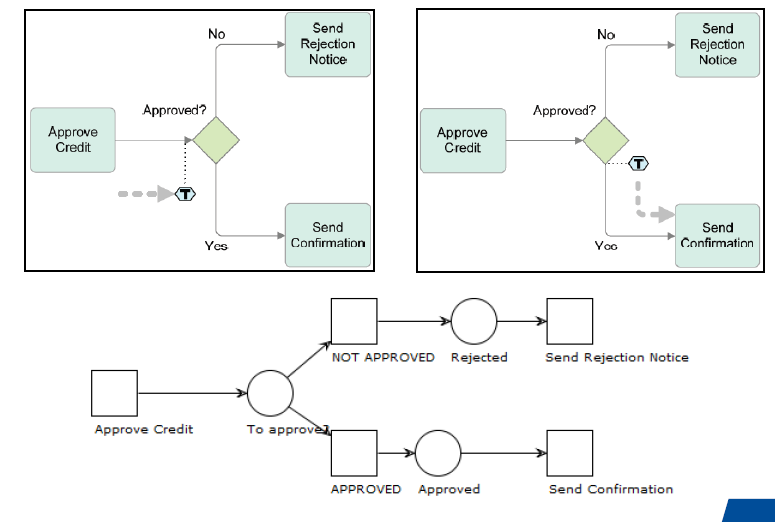
\includegraphics[width=0.75\linewidth]{capitolo 9/3.png}
\end{figure}

\subsubsection{XOR Join}

An XOR join merges multiple incoming branches into one. When a token reaches an XOR join, it waits for a token from one of the incoming branches before proceeding. This ensures that the process flow is synchronized and that no tokens are lost.
\begin{figure}[h!]
    \centering
    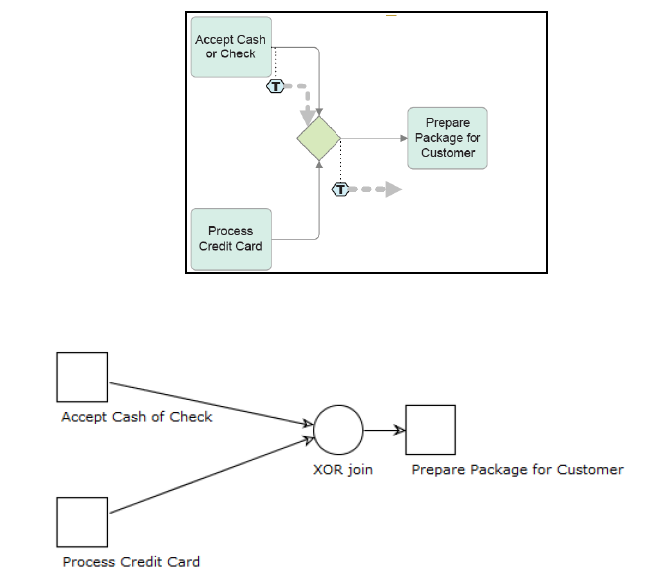
\includegraphics[width=0.75\linewidth]{capitolo 9/4.png}
\end{figure}
\newpage

\subsubsection{Default Condition}

In some cases, none of the conditions at an XOR split may be true, leading to a deadlock. To avoid this, a default condition can be introduced. The default condition is indicated by a slash (/) on the arc and ensures that if no other condition applies, the default condition will always be taken.
\begin{figure}[h!]
    \centering
    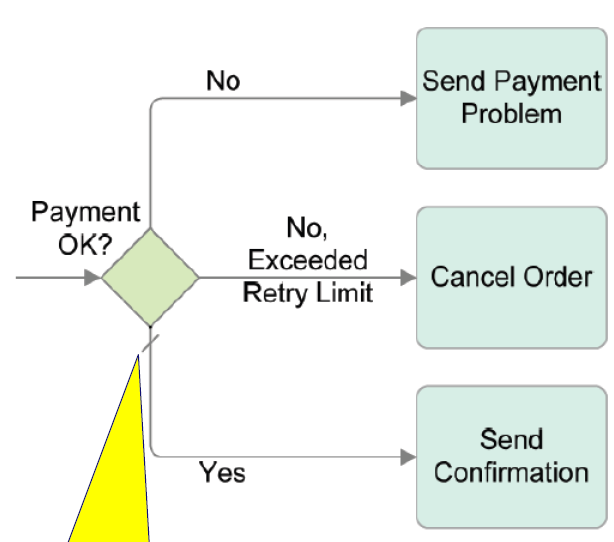
\includegraphics[width=0.5\linewidth]{capitolo 9/5.png}
\end{figure}

\subsection{Parallel Gateways (AND)}

Parallel gateways, also known as AND gateways, allow the process to split into multiple concurrent paths or merge multiple concurrent paths into one. Unlike exclusive gateways, parallel gateways do not evaluate conditions.

\subsubsection{AND Split}

When a token reaches an AND split, it is split into multiple copies, one for each outgoing branch. This allows multiple activities to be executed concurrently. An AND split can be modeled using Petri nets with black tokens, where each token represents a concurrent path.
\begin{figure}[h!]
    \centering
    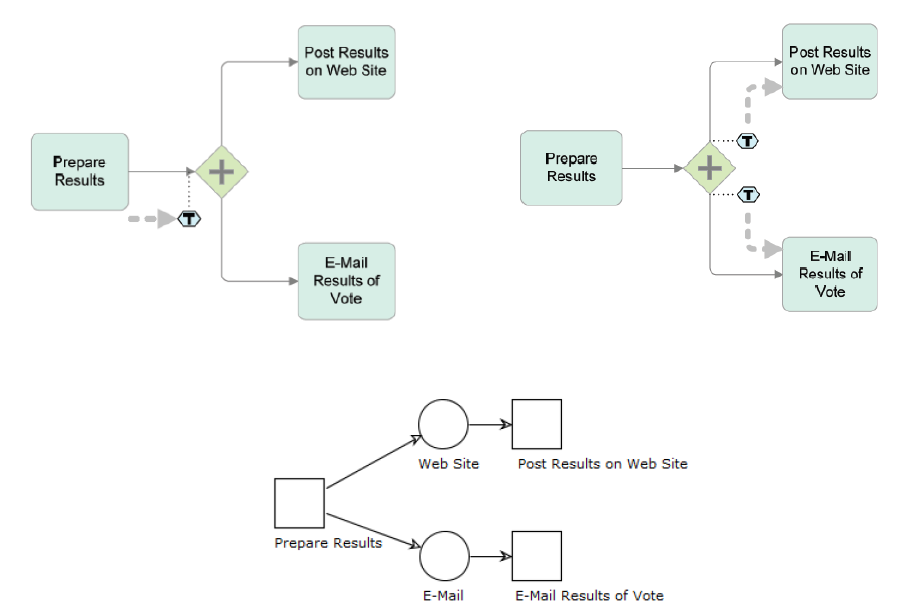
\includegraphics[width=0.75\linewidth]{capitolo 9/7.png}
\end{figure}
\subsubsection{AND Join}

An AND join waits for all incoming tokens before merging them into one token for the outgoing branch. When the first token arrives, it is held until all tokens arrive. Once all tokens have arrived, they are merged, and a single token is produced for the outgoing branch. This ensures that all concurrent paths are synchronized before the process continues.
\begin{figure}[h!]
    \centering
    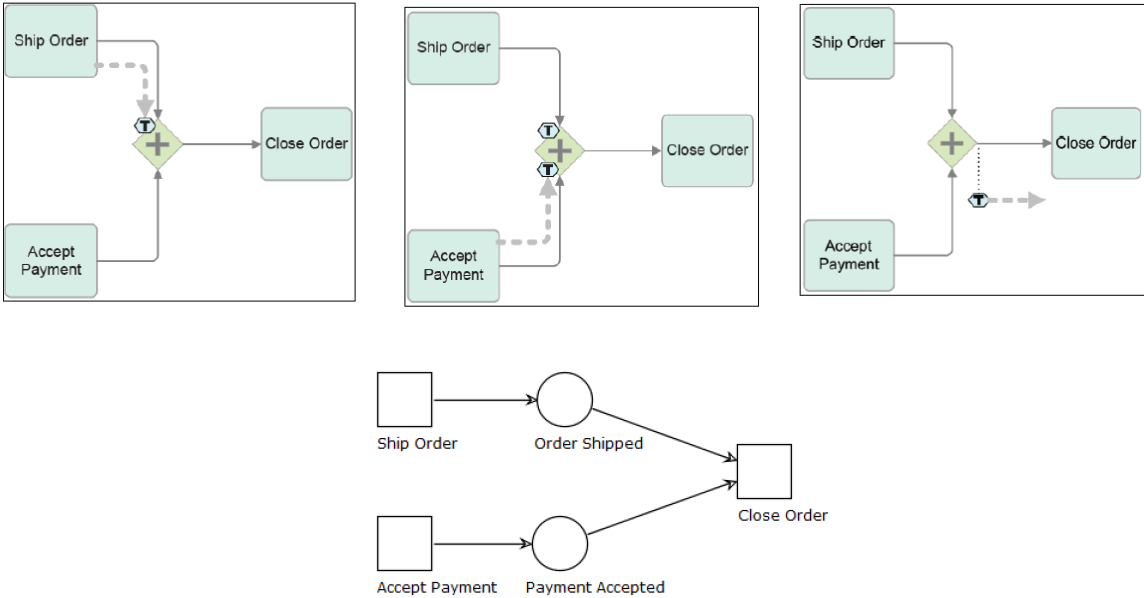
\includegraphics[width=0.75\linewidth]{capitolo 9/8.png}
\end{figure}

\subsection{Inclusive Gateways (OR)}

Inclusive gateways, also known as OR gateways, allow one or more branches to be activated based on certain conditions. The semantics of inclusive gateways lie between exclusive and parallel gateways.

\subsubsection{OR Split}

When a token reaches an OR split, it is consumed, and one token is produced for each condition that evaluates to true. To avoid deadlocks, it is assumed that at least one condition will evaluate to true. This ensures that the process flow can continue without interruption.
\begin{figure}[h!]
    \centering
    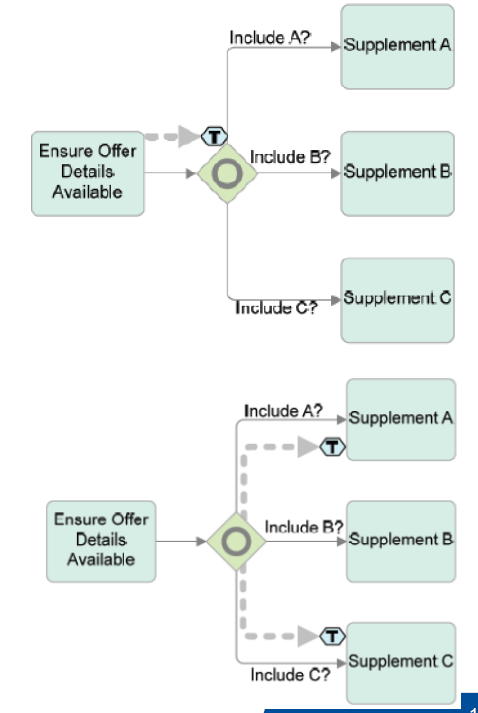
\includegraphics[width=0.75\linewidth]{capitolo 9/9.png}
\end{figure}
\subsubsection{OR Join}

An OR join waits for tokens from one or more incoming branches before merging them into one token for the outgoing branch. When the first token arrives, the gateway looks upstream to check if other tokens are expected. If another token is expected, the arrived token is held until all expected tokens arrive. Once all expected tokens have arrived, they are merged, and a single token is produced for the outgoing branch.

The behavior of an OR join is not local, as it requires looking upstream to determine if other tokens are expected. This makes it more complex than exclusive or parallel joins but allows for more flexible process flows.
\begin{figure}[h!]
    \centering
    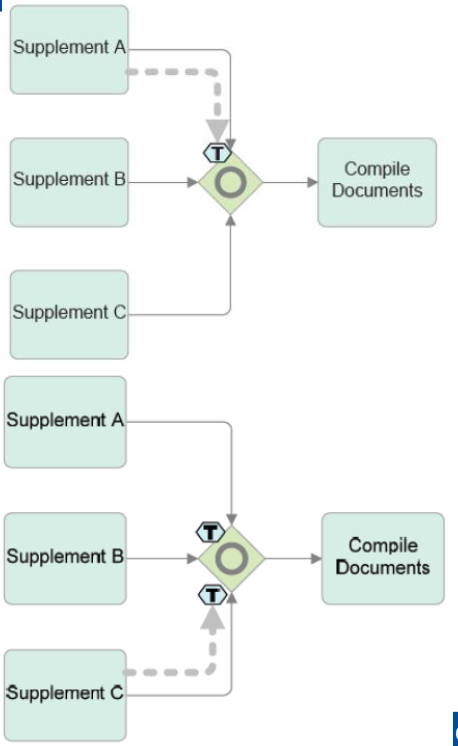
\includegraphics[width=0.75\linewidth]{capitolo 9/10.png}
\end{figure}
\section{Multiple End Events}

In BPMN, it is possible to have multiple end events within a single process. When one end event is reached, the execution can still continue to reach other end events. Each end event is mapped to a different end place in a Petri net, making it not a workflow net. However, multiple end events can be converted into a single end event to create a workflow net.
\begin{figure}[h!]
    \centering
    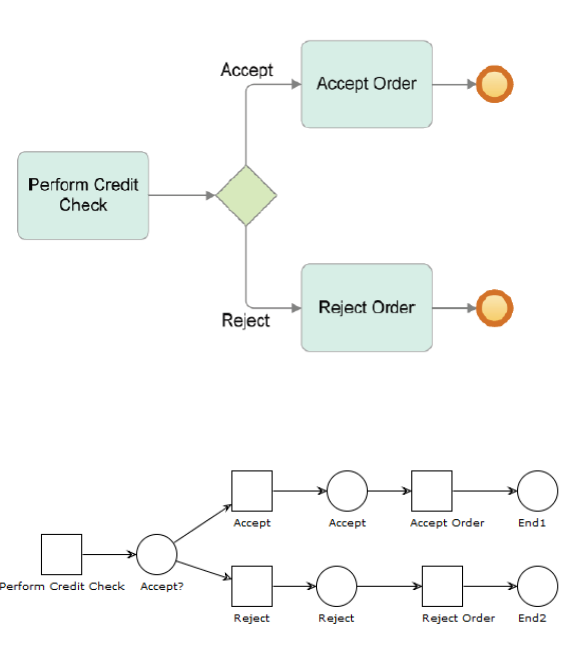
\includegraphics[width=0.75\linewidth]{capitolo 9/11.png}
\end{figure}

\section{Timer Intermediate Events}

Timer intermediate events indicate that an activity is enabled after a given delay. This allows for time-based triggers within the process. The mapping of timer intermediate events to Petri nets can only be informal, as Petri nets do not have time-related concepts.
\begin{figure}[h!]
    \centering
    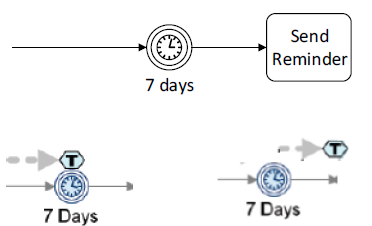
\includegraphics[width=0.75\linewidth]{capitolo 9/12.png}
\end{figure}
\newpage
\section{Terminate End Event}

A terminate end event causes the immediate cessation of all active branches of the process instance. This can be modeled in a Petri net by removing all tokens from the net, effectively stopping the process.
\begin{figure}[h!]
    \centering
    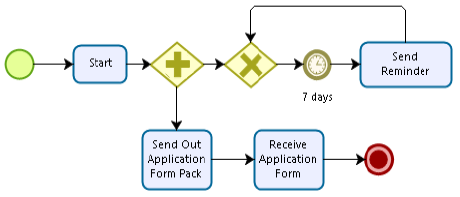
\includegraphics[width=0.75\linewidth]{capitolo 9/13.png}
\end{figure}

\section{Resources in BPMN}

Resources in BPMN can be captured using pools and lanes. Pools represent independent organizational entities, such as customers and suppliers, while lanes represent resource classes within the same organization. Communication between pools happens through message exchanges, while entities in different lanes can communicate directly.
\begin{figure}[h!]
    \centering
    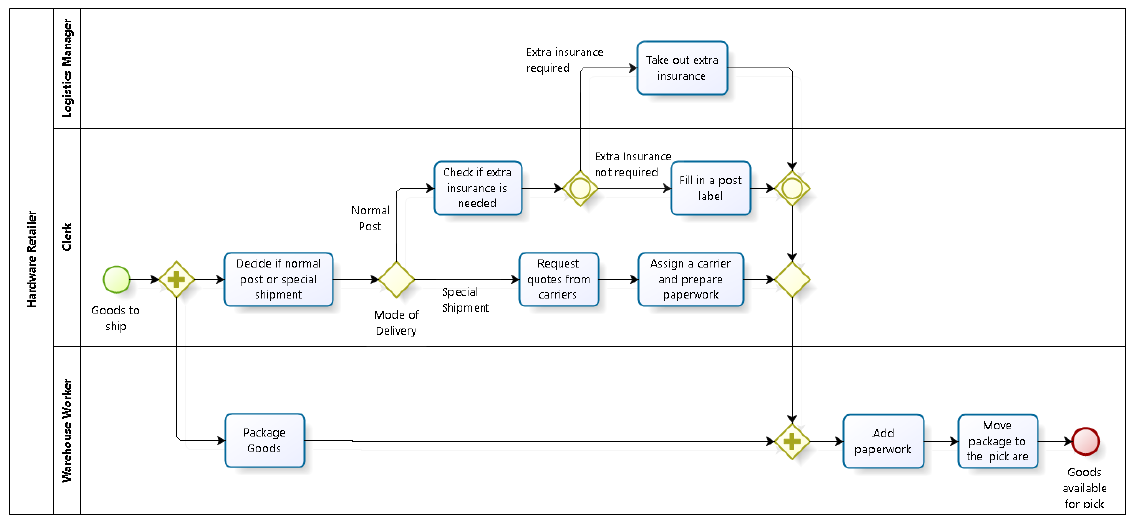
\includegraphics[width=0.75\linewidth]{capitolo 9/14.png}
\end{figure}
\newpage
\subsection{Messages}

Messages in BPMN define the communication between activities of two different pools. Messages cannot be exchanged between activities within the same pool, and sequence arcs cannot cross pool boundaries. Messages can also be sent to a pool without affecting its behavior, serving as informative notifications.
\begin{figure}[h!]
    \centering
    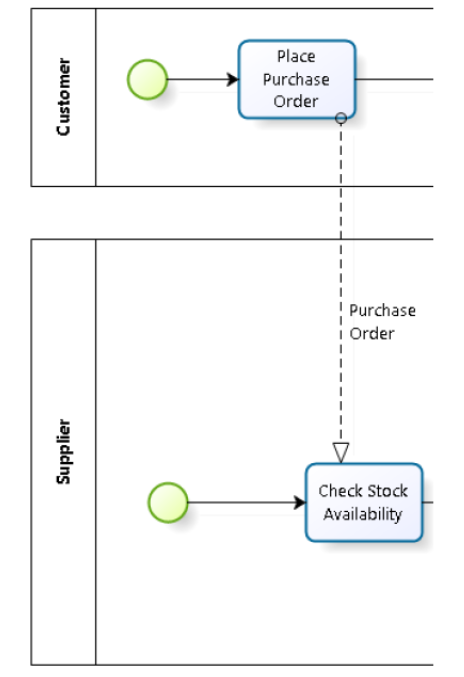
\includegraphics[width=0.5\linewidth]{capitolo 9/15.png}
\end{figure}
\subsection{Message Events}

Message events make the production and consumption of messages explicit within the process. When converting to Petri nets, each message event is represented as a place in the Petri net.
\begin{figure}[h!]
    \centering
    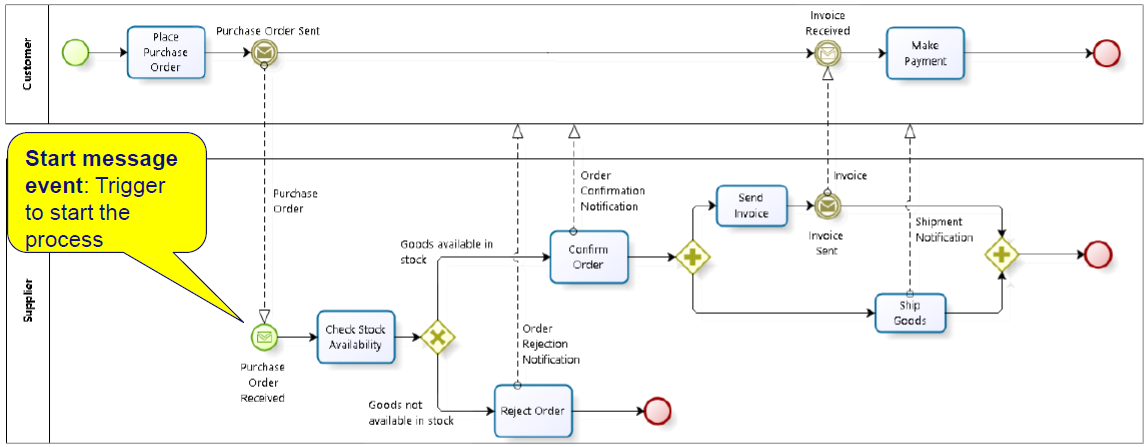
\includegraphics[width=0.75\linewidth]{capitolo 9/16.png}
\end{figure}
\section{Event-Based Exclusive Gateways}

Event-based exclusive gateways represent an alternative branching point where the decision is based on the occurrence of events rather than data-oriented conditions. The condition for branching is the reception of a message, making it different from traditional XOR gateways. This can be modeled in a Petri net by representing each event as a place in the net.
\begin{figure}[h!]
    \centering
    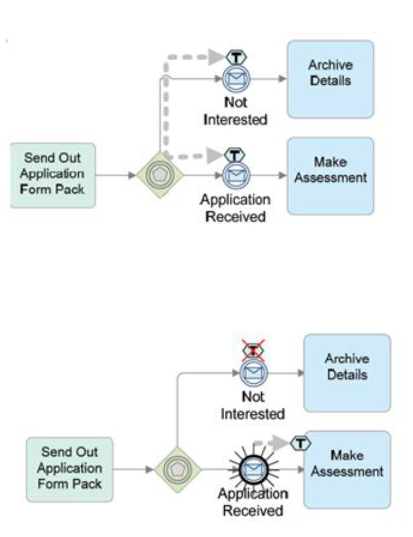
\includegraphics[width=0.5\linewidth]{capitolo 9/17.png}
\end{figure}

\section{Modeling Data in BPMN}

Data objects in BPMN are used to show how data and documents are used within a process as inputs and outputs of activities. A collection of data objects represents a collection of information, such as a list of ordered items. However, the support for data in the BPMN standard is limited. Data objects and collections are not typed and are not correlated with the activity's guards, such as at XOR or OR gateways.

Data objects may have states that depict how the object is updated within the process. Data flow represents the movement of data into and out of activities and is decoupled from the sequence flow. If data objects and collections have no state, black tokens can be used to represent them. If they have states, the activity producing the data can be duplicated for each state.

In conclusion, BPMN provides a comprehensive and standardized way to model business processes. Its key elements, including activities, events, gateways, and sequence flows, along with the concept of tokens, enable the creation of clear and consistent process diagrams. Understanding these elements and their semantics is crucial for effectively modeling and managing business processes.
\begin{figure}[h!]
    \centering
    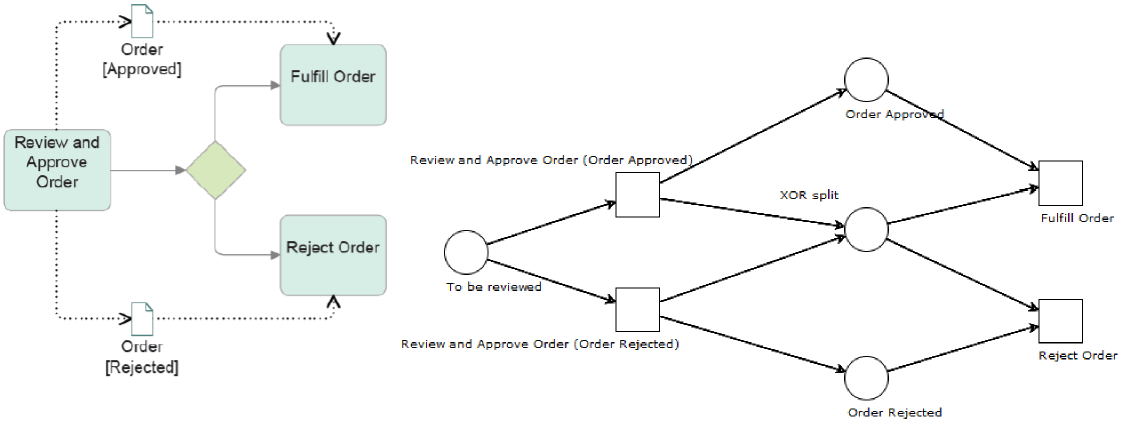
\includegraphics[width=0.75\linewidth]{capitolo 9/18.png}
\end{figure}